\section{RESULTADOS}

Apresentamos os resultados obtidos na comparação de diferentes modelos de aprendizado profundo na segmentação de feridas malignas em imagens médicas. Primeiramente, descrevemos o processo de criação do conjunto de dados clínicos e as técnicas de pré-processamento de imagens utilizadas. Em seguida, apresentamos os resultados de desempenho dos modelos, levando em consideração os resultados das métricas abordadas. Também realizamos uma análise comparativa entre os modelos e discutimos suas contribuições e perspectivas futuras. Esperamos que esses resultados possam contribuir para o desenvolvimento de ferramentas de diagnóstico e tratamento mais precisas e eficazes para pacientes com feridas malignas.

\subsection{Criação de um Dataset}

     O grande objetivo da criação de um novo dataset foi garantir a qualidade e confiabilidade dos dados, bem como a representatividade e variedade das imagens. Para isso, foram coletadas imagens de feridas malignas de diversas fontes, incluindo repositórios públicos no GitHub e sites especializados em imagens médicas. Essas imagens foram selecionadas com base em sua heterogeneidade, ou seja, foram escolhidas imagens que apresentam diferentes tipos de feridas malignas, tamanhos, formas e variações. Ao todo, foram selecionadas mais de 4.500 imagens para compor o conjunto de dados. Essas imagens foram pré-processadas antes do treinamento dos modelos, a fim de garantir a qualidade e confiabilidade dos dados. Além disso, foram especificadas as características das imagens, como resolução, dimensões e formato de arquivo, para proporcionar uma compreensão mais completa do conjunto de dados. Apresentamos os resultados obtidos com a criação do conjunto de dados exclusivo para a segmentação de feridas malignas, destacando a importância e o impacto dessa etapa no estudo.
    
    Qualidade e Confiabilidade: Este conjunto de dados foi construído com um processo meticuloso de coleta, pré-processamento e anotação. A inclusão de informações clínicas precisas aumenta consideravelmente a qualidade e confiabilidade desses dados. Isso os torna recursos inestimáveis para profissionais de saúde ao diagnosticar e tratar feridas malignas, proporcionando uma base sólida para desenvolver abordagens de segmentação mais eficazes.
    
    Representatividade e Variedade: Este conjunto de dados engloba uma ampla gama de tipos de feridas malignas, assegurando que os modelos criados possam lidar com a diversidade encontrada na prática clínica. A estratificação cuidadosa dos conjuntos de treinamento e teste garante uma representação equilibrada de cada classe de interesse, o que é fundamental para avaliar justamente o desempenho dos modelos. Isso promove a capacidade dos modelos de generalizar para diferentes casos clínicos.
    
    Fundação para Modelos de Aprendizado Profundo: O conjunto de dados estabelecido se destaca como uma base sólida para o desenvolvimento e teste dos modelos de segmentação de feridas malignas baseados em aprendizado profundo neste estudo. Sua qualidade excepcional e diversidade abrem caminho para o sucesso desses modelos, permitindo uma análise precisa e abrangente das técnicas de segmentação propostas.

    O conjunto de dados criado neste estudo é amplo e diversificado, o que contribui para aprimorar os resultados e desenvolver modelos de aprendizado profundo mais eficazes na segmentação de feridas malignas.

\subsection{Desempenho dos Modelos}

    % Os modelos de aprendizagem profunda deverão ser capazes de segmentar com sucesso as feridas malignas nas imagens médicas. A performance de cada modelo será avaliada utilizando métricas como acurácia, precisão, recall, F1-score e coeficiente de Dice.
    
    % Espera-se que todos os modelos apresentem bom desempenho, dada a capacidade das arquiteturas escolhidas para a tarefa de segmentação de imagem. Contudo, algumas diferenças no desempenho podem ocorrer devido às características específicas de cada arquitetura.
    
    Este estudo avaliou a eficácia de modelos de aprendizado profundo, especificamente \ac{FCN}, \ac{U-Net}, \ac{SegNet} e \ac{MobileNetV2}, na segmentação de feridas malignas em imagens médicas. A metodologia proposta gerou resultados significativos.
    
    \subsubsection{FCN}

        Os resultados indicam uma precisão notável em 150 épocas de treinamento, Com uma Precision de 0,9737, o modelo \ac{FCN} classificou corretamente cerca de 97,37\% dos pixels como pertencentes às áreas de feridas malignas, isso significa que a grande maioria dos pixels identificados como feridas malignas pelo modelo realmente fazia parte dessas áreas. Com o  Recall de 0,9527, o modelo foi capaz de identificar aproximadamente 95,27\% dos pixels que eram verdadeiramente partes de feridas malignas na imagem. Essa métrica destaca a capacidade do modelo em identificar uma grande parte das áreas de interesse, minimizando a omissão de pixels que eram feridas malignas. Coeficiente Dice de 95,87\%, representa a sobreposição entre a segmentação feita pelo modelo e a segmentação manual. Quanto maior esse valor, maior a semelhança entre as duas segmentações, No caso do desse modelo, houve uma alta concordância entre a segmentação prevista pelo modelo e a segmentação manual, indicando uma considerável sobreposição entre as áreas identificadas pelo modelo e as identificadas manualmente. Esses números refletem a capacidade do modelo em identificar com precisão as áreas de interesse nas imagens médicas, minimizando tanto os falsos positivos quanto os falsos negativos.
      
          \begin{figure}[H]
            \centering
            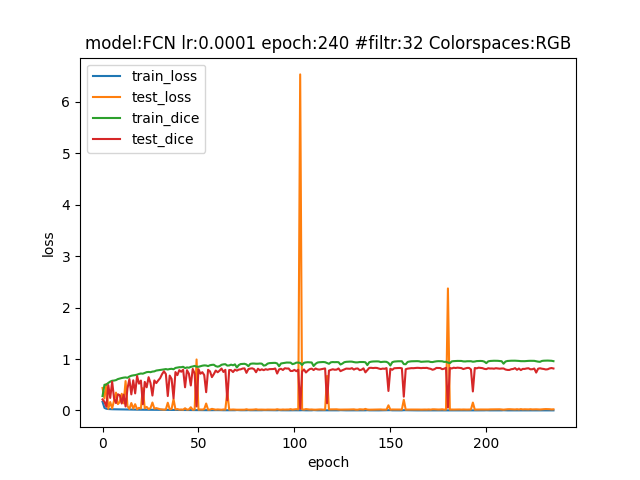
\includegraphics[width=0.8\textwidth]{img/fcnmodelfile.png}
            \caption{ Gráfico do Treinamento do Modelo \acf{FCN} }
            \label{fig:graphFCN}
          \end{figure}

        Na figura \ref{fig:graphFCN}, observamos a Loss associada ao FCN, que inicia ligeiramente acima de zero e se mantém relativamente estável, indicando a capacidade do modelo em aprender os padrões das imagens ao longo das épocas. No entanto, vale notar os picos nos valores de test loss por volta das 100 e 150 épocas, sugerindo momentos de desafio na generalização do modelo para dados não vistos durante o treinamento.

        O comportamento do train dice próximo a 1 durante as épocas indica uma excelente sobreposição entre a segmentação do modelo e a segmentação manual. Enquanto isso, a variação do test dice entre 0 e 1 nas primeiras 60 épocas, seguida por uma estabilização, sugere uma aprendizagem mais estável após a fase inicial.

        Esses resultados destacam a capacidade do \ac{FCN} em identificar e segmentar com precisão as áreas afetadas nas imagens médicas de feridas malignas, oferecendo uma representação visual detalhada e confiável das regiões de interesse para o diagnóstico e tratamento adequado.

          
    \subsubsection{U-Net}

        O desempenho do modelo \ac{U-Net} na segmentação de feridas malignas revelou resultados significativos. Após 150 épocas de treinamento, o modelo alcançou uma Precision de 0,9471, com essa precisão o modelo identificou corretamente cerca de 94,71\% dos pixels como pertencentes às regiões de feridas malignas, isso significa que a grande maioria dos pixels classificados como feridas malignas pelo modelo realmente pertencia a essas regiões. Com o Recall de 92,22\%, o modelo conseguiu identificar com precisão 92,22\% dos pixels que eram realmente partes de feridas malignas na imagem, essa métrica reflete a capacidade do modelo em capturar uma grande parte das áreas de interesse, minimizando a omissão de pixels que eram feridas malignas. O valor de 93,07\% para o Coeficiente Dice representa o nível de sobreposição entre a segmentação prevista pelo modelo e a segmentação manual, quanto maior esse valor, maior a semelhança entre as duas segmentações. Nesse caso, a sobreposição entre a segmentação prevista pelo modelo e a segmentação manual foi significativamente alta, indicando uma concordância considerável entre as áreas identificadas pelo modelo e as identificadas manualmente. Esses números demonstram a capacidade robusta do modelo em identificar com precisão as áreas de interesse nas imagens médicas, o que é crucial para o diagnóstico e tratamento preciso.
        
          \begin{figure}[H]
            \centering
            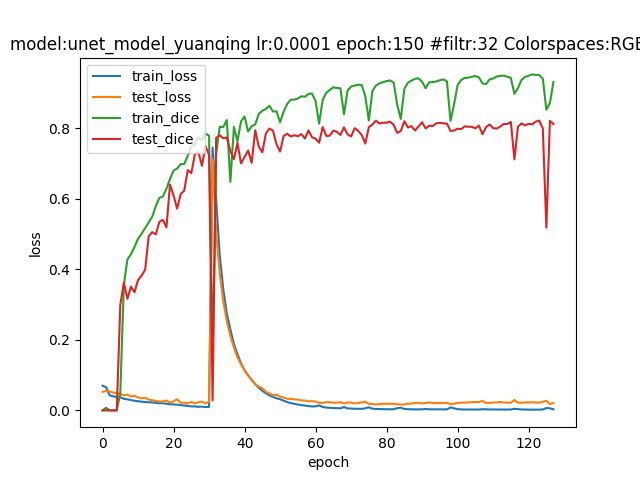
\includegraphics[width=0.8\textwidth]{img/unetprunedmodelfile.png}
            \caption{ Gráfico do Treinamento do Modelo \acf{U-Net} }
            \label{fig:graphU-Net}
          \end{figure}

        Observa-se na figura \ref{fig:graphU-Net}, que tanto o train loss quanto o test loss iniciam ligeiramente acima de zero, com um declínio rápido e um pico notável em torno das 35 épocas. Após esse pico, ambos os valores se estabilizam perto de zero, indicando que o modelo foi capaz de aprender eficazmente os padrões nas imagens de feridas malignas, mantendo uma baixa perda ao longo do treinamento.

        O comportamento do train dice começa em zero, mas rapidamente aumenta, estabilizando-se após aproximadamente 50 épocas, sugerindo uma aprendizagem estável e consistente na sobreposição entre a segmentação do modelo e a segmentação manual. O test dice apresenta comportamento semelhante, indicando uma capacidade relativamente alta de generalização para dados não vistos durante o treinamento, embora com valores ligeiramente inferiores.

        Esses resultados evidenciam a capacidade impressionante do modelo U-Net na identificação precisa das regiões de interesse nas imagens médicas de feridas malignas, oferecendo um desempenho consistente e confiável para aplicações clínicas.

          
    \subsubsection{SegNet}

        Os resultados obtidos pelo modelo \ac{SegNet} na segmentação de feridas malignas são bastante satisfatórios, embora ligeiramente inferiores aos modelos \ac{U-Net} e \ac{FCN}. Com uma precisão de 0,9247, o modelo classificou corretamente cerca de 92,47\% dos pixels como pertencentes às áreas de feridas malignas. Apesar de um pouco menor em comparação com os outros modelos, ainda indica uma boa capacidade do \ac{SegNet} em identificar as áreas de interesse. O Recall de 0,8787 indica que o modelo identificou aproximadamente 87,87\% dos pixels que eram realmente parte de feridas malignas na imagem. Embora seja um pouco menor em comparação com os outros modelos, ainda é um resultado aceitável, mostrando a habilidade do \ac{SegNet} em identificar uma parte significativa das áreas de interesse. O valor de 89,64\% para o Coeficiente Dice representa a sobreposição entre a segmentação feita pelo modelo e a segmentação manual.
        
          \begin{figure}[H]
            \centering
            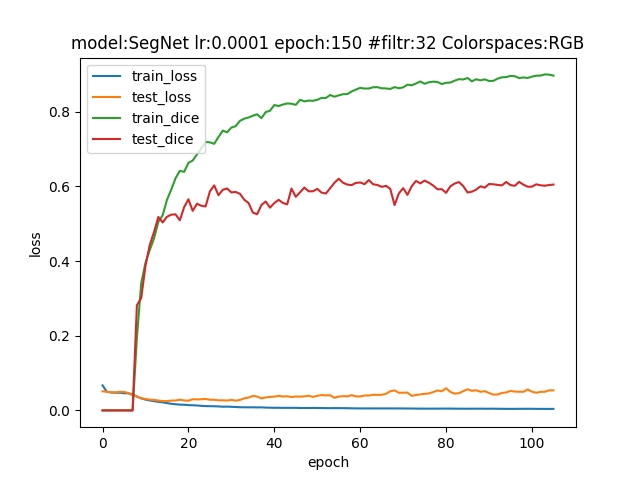
\includegraphics[width=0.8\textwidth]{img/segnetprunedmodelfile.png}
            \caption{ Gráfico do Treinamento do Modelo \acf{SegNet} }
            \label{fig:graphSegNet}
          \end{figure}

        Podemos verificar tambem na figura \ref{fig:graphSegNet} os valores de train loss, test loss, train dice e test dice ilustrando a evolução do treinamento do modelo, mostrando a estabilização das métricas após um certo número de épocas, o que é indicativo da convergência do modelo e da estabilização do seu desempenho.

          
    \subsubsection{MobileNetV2}

        Os resultados obtidos pelo \ac{MobileNetV2} na segmentação de feridas malignas são consideravelmente inferiores em comparação com os outros modelos. Com uma Precision de apenas 73,09\% é obtido um resultado consideravelmente mais baixo em comparação com os outros modelos, indicando que o \ac{MobileNetV2} teve dificuldades em identificar corretamente as áreas de interesse. Com Recall de 62,19\% e o Coeficiente Dice de 62,61\% podemos ver que o modelo não conseguiu alcançar uma similaridade satisfatória entre as áreas identificadas por ele e as identificadas manualmente.
    
          \begin{figure}[H]
            \centering
            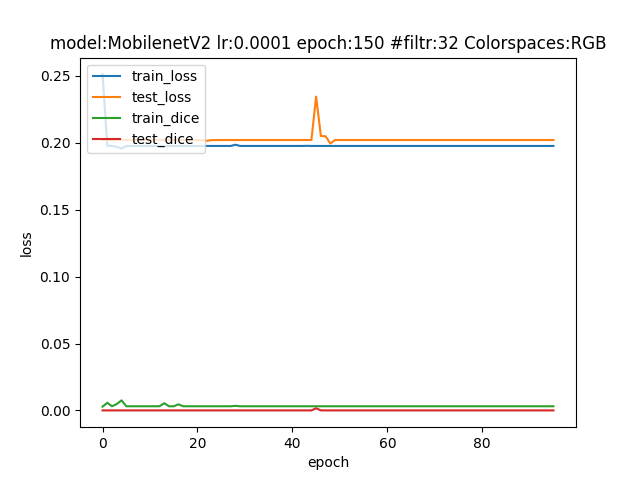
\includegraphics[width=0.8\textwidth]{img/mobilenetv2prunedmodelfile.png}
            \caption{ Gráfico do Treinamento do Modelo \acf{MobileNetV2} }
            \label{fig:graphMobileNetV2}
          \end{figure}

        Na figura \ref{fig:graphMobileNetV2} é exibidos os valores das métricas usadas no treinamento mostram que o modelo apresentou valores significativamente mais altos de perda e uma variação considerável das métricas de desempenho ao longo das épocas, indicando instabilidade no aprendizado.

        No geral, os resultados do \ac{MobileNetV2} foram consideravelmente inferiores em comparação com os outros modelos, demonstrando que ele não é adequado para essa tarefa específica de segmentação de feridas malignas em imagens médicas.
    
\subsection{Análise Comparativa Entre os Modelos}

    Na comparação dos modelos \ac{FCN}, \ac{U-Net}, \ac{SegNet} e \ac{MobileNetV2} para a tarefa de segmentação de feridas malignas em imagens médicas, alguns insights valiosos emergem. Cada modelo apresenta características distintas que podem influenciar a escolha do mais apropriado, dependendo das necessidades específicas do contexto clínico e dos recursos disponíveis.

    \begin{itemize}
        \item O \ac{FCN}, com sua alta precisão, Recall e Coeficiente Dice, demonstrou ser uma escolha sólida para aplicações que exigem detecção precisa das áreas afetadas. Sua capacidade de identificar regiões de interesse com pouca perda de informação é notável. O \ac{U-Net} também se destacou, oferecendo um desempenho igualmente impressionante. Ambos os modelos são altamente recomendados quando a precisão é de suma importância.

        \item O \ac{SegNet}, embora ligeiramente abaixo do \ac{FCN} e \ac{U-Net} em termos de métricas de avaliação, ainda apresentou resultados satisfatórios. Para aplicações onde os recursos computacionais são limitados, o \ac{SegNet} pode ser uma escolha mais eficiente, uma vez que seu desempenho é respeitável, e sua arquitetura é menos complexa.

        \item Por outro lado, o \ac{MobileNetV2} se destacou negativamente nesta comparação. Seus resultados significativamente inferiores indicam que, para a segmentação de feridas malignas, ele não é a escolha adequada. Este modelo é ineficaz na tarefa, demonstrando a importância de selecionar cuidadosamente a arquitetura do modelo em aplicações clínicas críticas.
    \end{itemize}
    
     \begin{figure}[H]
            \centering
            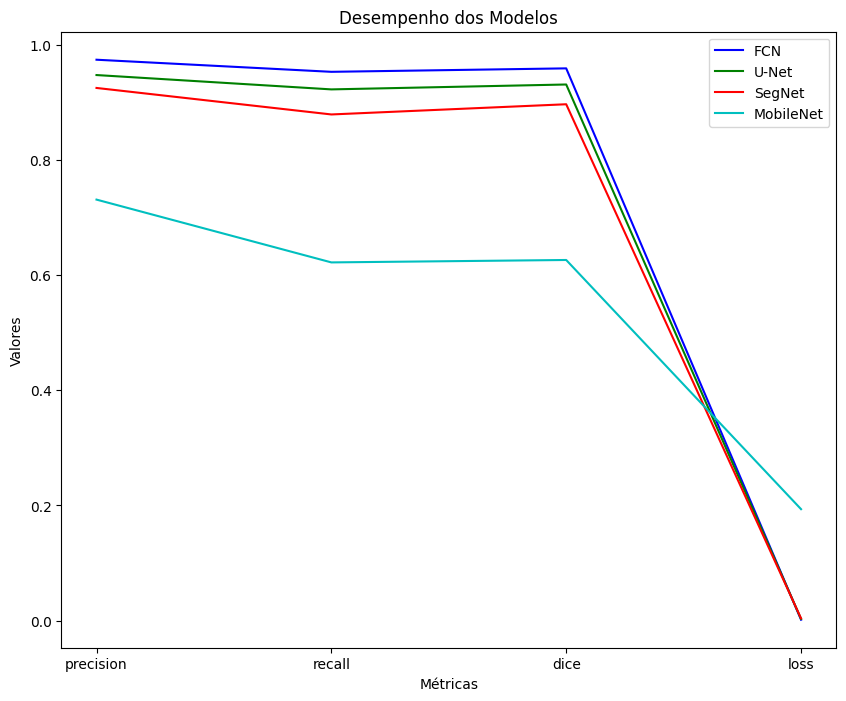
\includegraphics[width=0.8\textwidth]{img/results_metrics_models.png}
            \caption{ Comparação das Métricas dos Modelos Avaliados }
            \label{fig:graphResultsModels}
     \end{figure}

     \begin{enumerate}
        \item Na figura \ref{fig:graphResultsModels} é apresentado o gráfico comparativo dos modelos. podemos observar que as métricas Precision, Recall e Coeficiente de Dice apresentam valores mais altos para o modelo \ac{FCN} em comparação com os outros modelos. Isso indica que o modelo \ac{FCN} teve um desempenho melhor na segmentação. Além disso, a métrica Loss apresenta um valor mais baixo para o modelo \ac{FCN}, o que indica também que o modelo teve um menor erro na segmentação das feridas malignas.
    \end{enumerate}
    
    \begin{table}[htbp]
        % \tiny
        \centering
        \begin{tabular}{|l|l|l|l|l|l|l|}
            \hline
            Modelos   & Epochs & Precision & Recall  & Dice    & Loss      \\ \hline
            \ac{FCN}       &  150   & 0.9737    & 0.9527  & 0.9687  & 0.0017    \\ \hline
            \ac{U-Net}     &  150   & 0.9471    & 0.9222  & 0.9307  & 0.0030    \\ \hline
            \ac{SegNet}    &  150   & 0.9247    & 0.8787  & 0.8964  & 0.0040    \\ \hline
            \ac{MobileNetV2} &  150   & 0.7309    & 0.6219  & 0.6261  & 0.1936    \\ \hline
        \end{tabular}
        \caption{Análise Comparativa das Métricas dos Modelos Avaliados}
        \label{tab:analiseMetricas}
    \end{table}

    \begin{enumerate}
        \item A tabela ~\ref{tab:analiseMetricas} representa os resultados das métricas 
        dos modelos comparados. Os resultados obtidos mostraram que tivemos 2 modelos com maior precisão, o modelo \ac{FCN} apresentou a melhor performance, com valores de Precision, Recall, Coeficiente de Dice e Loss de 0.9737, 0.9527, 0.9687 e 0.0017 respectivamente. O modelo \ac{U-Net} também apresentou resultados promissores, com valores de Precision, Recall, Coeficiente de Dice e Loss de 0.9471, 0.9222, 0.9307 e 0.0030, respectivamente. A utilização dessas métricas é importante para avaliar a qualidade dos resultados obtidos pelos modelos e compará-los com outros modelos existentes na literatura. Os resultados obtidos neste estudo mostram que a utilização de modelos de aprendizado profundo pode ser uma abordagem eficiente para a segmentação de feridas malignas em imagens médicas. 
    \end{enumerate}
    
    \begin{table}[H]
    % \tiny
    \centering
    
    % \begin{figure}[H]
            \centering
            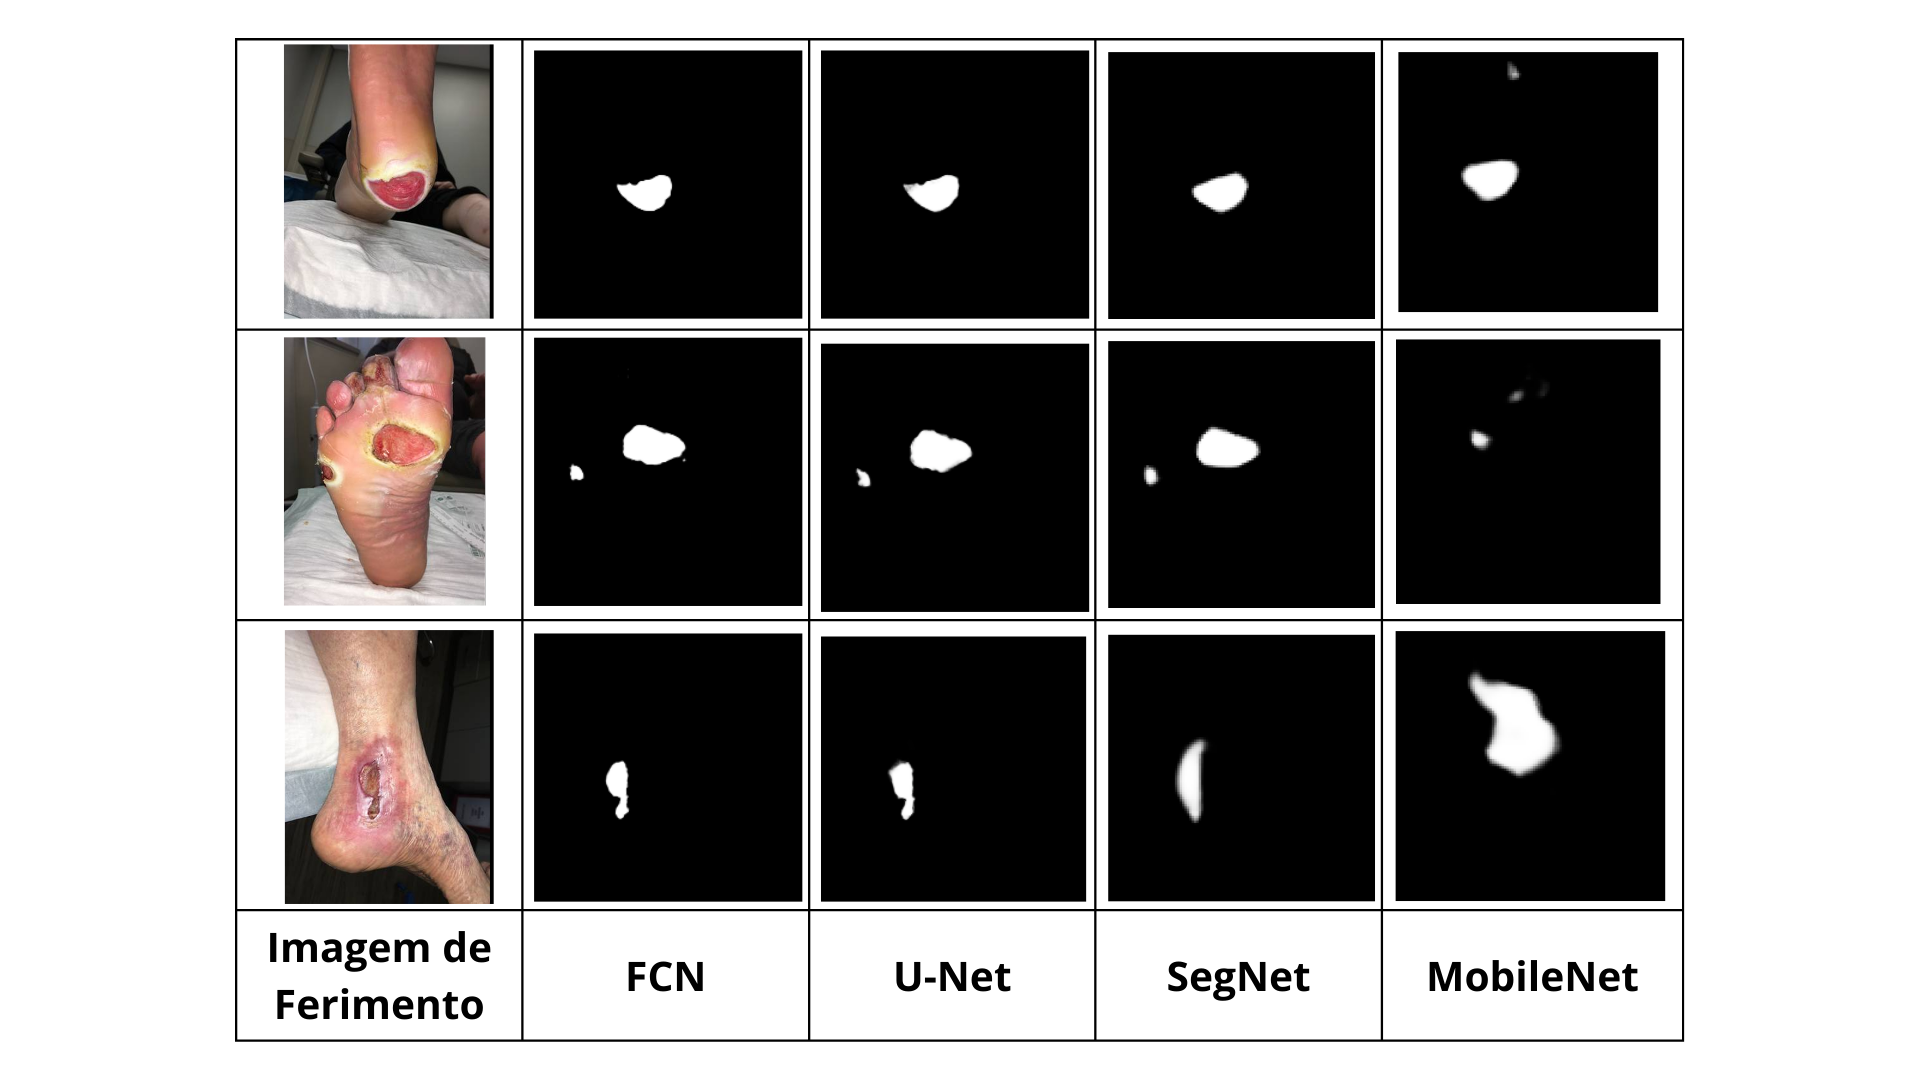
\includegraphics[width=0.8\textwidth]{img/resultado_segmentacao_modelos.png}
            \caption{ Resultado segmentação dos modelos }
            \label{fig:resultSegmetationModels}
     % \end{figure}
    
    \end{table}

    \begin{enumerate}
        \item Como podemos verificar na tabela \ref{fig:resultSegmetationModels} temos alguns exemplos do resultado da segmentação de 3 imagem da nossa base de dados para cada modelo avaliado, podemos verificar que o modelo \ac{FCN} se destacou em termos de precisão na segmentação, conforme mostrado em sua coluna. Sua abordagem de convolução total é altamente eficaz na captura de detalhes, tornando-o uma escolha sólida quando a máxima precisão é necessária em aplicações clínicas. O modelo \ac{U-Net} também se destacou em termos de precisão na segmentação de feridas. Sua capacidade de segmentação detalhada é adequada para aplicações clínicas que exigem a máxima precisão na identificação de feridas malignas. O modelo \ac{SegNet}, embora não alcance o mesmo nível de precisão que o \ac{FCN} e o \ac{U-Net}, ainda oferece resultados aceitáveis na segmentação das feridas. Por outro lado, o \ac{MobileNetV2} não obteve resultados satisfatórios na segmentação. Seus resultados significativamente inferiores indicam que não é uma escolha adequada para essa tarefa em aplicações clínicas críticas.
    \end{enumerate}

    Em resumo, a comparação entre os modelos revelou que \ac{FCN} e \ac{U-Net} são superiores em precisão e sensibilidade, tornando-os adequados para aplicações que exigem alta precisão em segmentação. O \ac{SegNet} oferece um equilíbrio entre desempenho e complexidade computacional, enquanto o \ac{MobileNetV2} não se mostrou eficaz. A escolha do modelo mais apropriado para a segmentação de feridas malignas em imagens médicas deve ser baseada nas necessidades específicas da aplicação clínica em questão. Se a prioridade é a máxima precisão, o \ac{FCN} e o \ac{U-Net} são escolhas sólidas. Para cenários com recursos computacionais limitados, o \ac{SegNet} pode ser uma alternativa aceitável. A seleção do modelo deve ser cuidadosamente ponderada em relação aos objetivos clínicos, à disponibilidade de recursos e à precisão desejada. Em última análise, a comparação entre esses modelos oferece uma base sólida para tomar decisões informadas na área de segmentação de feridas malignas em imagens médicas. 

\subsection{Contribuições e Perspectivas Futuras}

    Os resultados deste estudo prometem contribuir para o campo da oncologia cutânea, melhorando o diagnóstico e acompanhamento de feridas malignas. Além disso, fornecem insights para futuras pesquisas em aprendizado profundo aplicado à segmentação de imagens médicas, indicando caminhos para aprimorar modelos existentes ou desenvolver novas arquiteturas.

    Identificamos limitações e sugerimos direções promissoras para pesquisas futuras, como a necessidade de testar os modelos sob diversas condições para verificar sua robustez e a obtenção de um leque mais amplo de imagens em parcerias com instituições médicas.

    As contribuições deste estudo são significativas para a comunidade médica, pois oferecem ferramentas eficazes na segmentação de feridas malignas, o que pode levar a diagnósticos mais precisos e tratamentos mais eficientes. As perspectivas futuras incluem aprimorar ainda mais as abordagens propostas, ampliar a generalização e a aplicabilidade dos modelos em uma gama mais diversificada de cenários clínicos e explorar novas técnicas de aprendizado profundo para melhorar ainda mais a segmentação de feridas malignas em imagens médicas.

    Em síntese, esta pesquisa revelou resultados encorajadores na segmentação de feridas malignas em imagens médicas, proporcionando insights valiosos que orientarão investigações subsequentes. As contribuições deste estudo são notáveis para a comunidade médica, e as perspectivas futuras envolvem a otimização contínua das abordagens propostas, bem como a exploração de novas técnicas de aprendizado profundo para aprimorar ainda mais a precisão na segmentação de feridas malignas em imagens médicas.